\documentclass[12pt]{article}
\usepackage{color}
\usepackage[linesnumbered,ruled]{algorithm2e}
\usepackage{graphicx}

\SetKwInOut{Input}{Input}
\SetKwInOut{Output}{Output}
\SetKwProg{Fn}{Function}{}{}
% Allow really sloppy paragraphs that do not generate overfull or
%    underfull hbox's
\newenvironment{SLOPPY}{\begin{sloppypar}\hbadness=10000}{\end{sloppypar}}

\newcommand{\comment}[1]{\textcolor{red}{\it{#1}}}

\addtolength{\textwidth}{1.0in}
\addtolength{\oddsidemargin}{-0.5in}
\addtolength{\evensidemargin}{-0.5in}
\addtolength{\textheight}{1.5in}
\addtolength{\topmargin}{-0.8in}

\newcommand{\blankline}{\vspace*{\baselineskip}}

%\title{Ensemble Pipeline for Discovery of Motifs}
\title{Motif Combining and Association Tool: MCAT}

\author{Jeff Robertson, Jake Martinez, Yanshen Yang, Zhen Guo,\\
Christy Coghlan, Silke Hauf, Lenwood S. Heath}

\begin{document}
\maketitle

\begin{abstract}
\label{section:abstract}
% define problem and give motivation
%Motivation, Results, Availability and Implementation, Contact and Supplementary Information
\noindent
Motivation:
\textit{De novo} motif discovery in biological sequences is an important and
computationally challenging opportunity.
A myriad of algorithms have been developed to solve this problem with varying
success, but it can be difficut for even a small number of these tools to reach
a consensus.
Because individual tools can be better suited for specific scenarios,
an ensemble tool that
combines the results of many algorithms can yield a more confident and complete
result.\\
Results:
Orange Pipeline is an ensemble pipeline for discovering and ranking motifs in
DNA sequences.
It utilizes industy standard motif finding software to filter the sequences
and perform de novo motif discovery.
%It uses several novel techniques to cluster and score
%the results.
It then uses a novel motif comparing algorithm to combine the results and report
the top motifs, and visualise their locations and scores.\\
Availability: Orange Pipeline is open source and available at \_\_\_\_.\\
Contact: ...\\
Supplementary Information: ...
\end{abstract}

\section{Introduction}
\label{section:introduction}
Gene expression is governed by transcription factors that bind to short
sequences of DNA called motifs found in the promotor region of genes. % plurals mismatch?
The presence of similar motifs can imply coregulation of genes.
In the past, transcription factor binding sites have been found experimentally,
but this can be a slow and expensive process. \comment{citation}
If a gene's promoter region has been sequenced, motifs can be found
computationally and confirmed by experiment, making the process of motif
identification significantly more efficient. \comment{possible citation,
    many publications for individual tools, few about \it{in silico} motif
finding in general}
The orange pipeline was originally inspired by the study of six genes in
fission yeast.% Schizosaccharomyces pombe.
These genes are associated with the yeast cell cycle
in particular, 
the spindle assembly checkpoint (SAC)
\cite{He22071997}\cite{Kim1045}
\comment{relevant, but old articles, possibly get more recent publications
from Dr. Hauf? easier to find sources for budding yeast, hard to tell
how relevant they are}, 
and are believed to be co-regulated,
implying that their promoter regions might contain similar motifs.
The pipeline seeks these motifs by running well-established motif
discovery tools on the provided data then combining and reporting the results
using novel techniques explained later.

\begin{SLOPPY}
This pipeline combines several standard tools and some novel
techniques. The tools we have used were carefully selected for both breadth
and depth of algorithms used. We chose five motif finding tools
that cover a broad range of discovery and validation approaches so the
pipeline can find a motif even
if several of the individual tools are incapable of discovering it.
Furthermore, if a similar motif is found by all or most of the tools, we are
all the more confident in that motif being a good result.
%\comment{Include citations
%to ensemble tools compared to later}\\
\end{SLOPPY}

\section{Methods}
\label{section:methods}

\subsection{Overview}
\label{section:Overview}
\begin{SLOPPY}
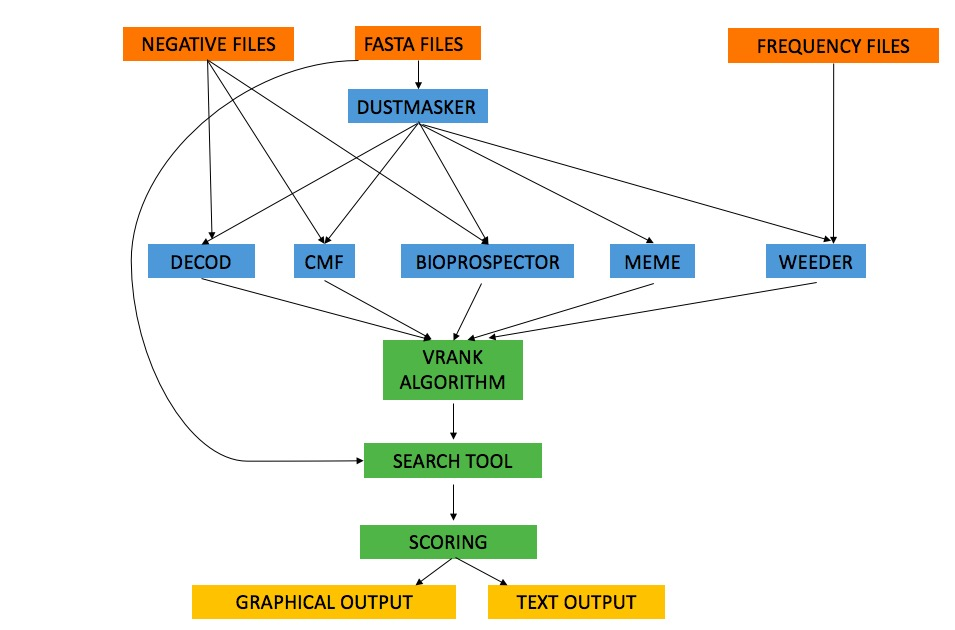
\includegraphics[scale=.4]{mcat_ensemble_v1.jpg}\\
The pipeline consists of several stages. First, the input files are
filtered for low complexity regions. Once these regions are found and masked,
the pipeline runs multiple  motif discovery tools in parallel.
The results from these tools are collected and scored against
each other.
The original input files are searched for instances of the top scoring results.
Based off these instances, the pipeline calculates statistical scores
for each of the top results
and visualizes them.\\
\end{SLOPPY}

\begin{SLOPPY}
Motif Discovery Tools\\

\indent
DustMasker \cite{citeulike:7471857} is used to filter out low complexity
regions from motifs.
The FASTA file provided as input to the pipeline is first run through
DustMasker, which finds and marks low complexity regions. Any marked nucleotides
are then replaced with 'N' to indicate that they should not be considered as a
possible part of a motif.\\
\end{SLOPPY}

\begin{SLOPPY}
MEME \cite{pmid7584402} was chosen for motif discovery because it
is possibly one of the most commonly used tool in this area. Our own test
results have validated this choice, showing that MEME often contributes 
significantly to results. % include preliminary test statistics
MEME uses multiple expectation maximizations to elicit possible motifs from the
input data. It records each result, then masks them out allowing MEME to find
additional motifs without being distracted by motifs that have already been
found.
It is run with mostly default parameters, only specifying motif width,
number of motifs to search for, and input format.
\\
\end{SLOPPY}

\begin{SLOPPY}
CMF \cite{Lee01092013} \cite{Mason15112010} is also used for motif discovery.
It utilizes motif seeding to contrast a set of sequences believed to contain
the desired motif and a negative set. The results are then derived from the
motifs that are found to be over represented in the positive sample.
% reword next sentence
The pipeline uses the desired motif width to set 
the motif length parameters for CMF. The lower bound is the
target motif length minus two, the upper bound is the target motif length plus
two, and the seed length is equal to the target motif length.
\\
\end{SLOPPY}

\begin{SLOPPY}
BioProspector \cite{Liu01bioprospector:discovering} uses Gibbs sampling to
find motifs. This is a random algorithm and the implementation in BioProspector
allows for gapped motifs and motifs containing palindromic patterns.
% Unnecessary detail?
BioProspector requires its input to be in a restricted FASTA file format, so
the filtered FASTA file is passed through a converter before it is the imput to
BioProspector.
It is run with default parameters.
% no longer true, added -w, needs testing
\\
\end{SLOPPY}

\begin{SLOPPY}
DECOD \cite{Huggins01092011} finds motifs in a way that is somewhat similar
to CMF, but it uses $k$-mer counts instead of motif seeding. By default it is
run with fifty iterations, a sequence cardinality of 5, and is set to look for
three motifs.
\\
\end{SLOPPY}

\begin{SLOPPY}
Weeder \cite{Pavesi01072004} is a common motif finding tool.
% cite Tompa et al. for inluence in choice
It exhaustively enumerates possible consensus sequences determined from
precomputed frequency files, evaluating each one against
the sequences from the FASTA file. It does this multiple times with differing
motif lengths and number of substitutions allowed, then reports the top 
results. Weeder is run with frequency files generated from the genome being
studied. These can be created with the w2frequency\_maker program provided
by weeder which is included with MCAT under the weeder folder.
The maxm parameter is set so that it
returns a maximum of ten results.
% Weeder needs accurate freq files, where should it get them?
\\
\end{SLOPPY}

\noindent
\begin{SLOPPY}
\comment{Include whether each tool can handle 0 or more than
one instances per
sequence or gapped motifs}\\
\end{SLOPPY}

\noindent
\subsection{Novel Tools}
\begin{SLOPPY}
\comment{these need better names}\\

\noindent
Combining Results\\
MCAT uses an algorithm named VRank to combine the results from each of the
motif discovery tools. VRank first conducts a poll, letting each tool vote
for the
positions where it found a motif. The algorithm then enumerates through the
positions of the original results, keeping a sum of the number of votes found
within instances of
each result. The motifs are then ranked by this score and the top three results
which are not too similar are chosen.\\
\end{SLOPPY}

\begin{SLOPPY}
\noindent
Search for results\\
The search tool takes the three top results and searches for them in the
original FASTA file. It does this by looking at every position in each DNA
sequence and returning any instances it finds that have one of the top three
comparison scores to the motif. For motifs that are well conserved, this
can return a surprisingly large number of results.\\
\end{SLOPPY}

\begin{SLOPPY}
\noindent
Scoring results\\
A myriad of scores are computed for each of the three results. These include
the comparison score described above which by itself only reflects on motif
quality compared to other comparison scores from within the same run of the
pipeline but taken together can indicate how strongly the various tools were
in agreement about this result.
The pipeline also reports the log likelihood
for the position weight matrix of each motif based on the background nucleotide
ratios in the FASTA file [citation needed].
Other scores reported by the pipeline are the P-value, Z-Score, and Q-value.
[citations needed]
\\
\comment{Include Jake's writeup on p-values and
fill in scoring details once they are decided}\\
\\
P-value with QFAST\\
MCAT is designed to calculate the P-value for one motif against a set of target sequences. QFAST algorithm [citations needed] uses the P-value for each sequence and then combine them.  In each target sequence, the Markov-chain probability score is calculated for all possible candidate motifs. The position P-values are the probability of observing a match score at least as good from a random sequence. The sequence P-value is either from the exact match candidate motif or from combined P-value of the  candidate motifs which are similar to the query motif . If no similar motifs are found under the similarity of 80\%, the sequence P-value is set to 1.0. Then QFAST generates a combined P-value from the product of all the sequence P-values. This combined P-value indicated the probability that the query motif appears in the total set of sequences compared to a random set of sequences.\\

\end{SLOPPY}

\subsection{Benchmark Data} 
\begin{SLOPPY} 
MCAT was tested with both synthetic and real data sets. The synthetic data sets were 
created with our tool, \verb|seq_gen.py|, and had motif length of 5-12 nucleotides, 
1-3 motifs, and a sequence length of 500, 800, and 1000. We used the same E. coli 
genome that EMD did to test our ensemble. The set of motif groups, ECRDB62A, had 
1.85 average sites per sequence, 12 average number of sequences per motif group, 
an average site width of 
22.83, and an average sequence length of 300 nucleotides. 
%currently just using the same test data as EMD did so the stats are the same
%could change to S. Pombe
\\ 
\end{SLOPPY}

\section{Comparison with existing tools}
\label{section:comparison}

\noindent
\subsection{Overview of Similiar Tools}

\begin{SLOPPY}
\indent
%include pros/cons of MCAT?
The vast majority of similiar ensembls use tools that rely on a  Markov model (such as 
GimmeMotifs, MEME-ChIP, and Peak-motifs). Additionally, most compare the 
results against a database such as JASPAR
(Melina II) or STAMP (CompleteMOTIFs). Some pipelines, such as Tmod and 
Melina II, do not perform any statistical analysis on the motif results and 
simply allow the user to run the results through an external tool. Most 
pipelines take in FASTA for ChIP-Seq data, and many limit the number of input
sequences.\\

%EMD overview
One ensemble tool, EMD \comment {citation needed}, works to make it simple to implement new component algorithms 
into the ensemble and is made to run on distributed computer systems.  The sites that each algorithms predicts are grouped 
by the score that each algorithm gives them. Motifs that are in a top group as part of most 
of the algorithms are identified (all of the predicted sites are given equal weights). The number of times a position in 
the sequence is identified is counted and a sliding window is used to smooth the score and decide the final site prediction. 
It works by running the algorithms multiple
times, often with different paramaters, in order to achieve diverse predictions. \\

%DynaMIT overview
Another ensemble tool, DynaMIT \comment {citation needed}, is completely customizable. It allows users to use whichever motif finding algorithms, combinations, and results printers that they choose. In the paper, DynaMIT was often tested by running MEME and GLAM2 or Weeder on the sequences, then running the results from each algorithm through novel combining methods, known as integration strategies, such as Jaccard, MutualInformation, and PCA (Principal Component Analysis). 
\end{SLOPPY}

\subsection{Comparison With Other Tools}
\begin{SLOPPY}
\indent

%working ensembles
We compared MCAT against several similiar ensemble tools. The first, EMD, discussed above, is available as a downloadable
from its website. We ran it against the test data, both synthetic and ECRDB62A (which originally came from EMD's authors). For all runs, it EMD
was configured to find the top 5 motifs of width 15. \\
\comment {results of EMD}

We also tested against DynaMIT, a comprable ensemble that is detailed above. We ran the test data using MEME and GLAM2 as the algorithms and Jaccard, MutualInformation, and PCA as the integration strategies, much like the DynaMIT paper had done.\\ 
\comment {results of DynaMIT}

%non-working ensembles
Of the ensembles that use FASTA files as input, most are close to a decade old. Because of these, we were unable
to test against several comprable pipelines. One such ensemble, MotifVoter, notably allows users to choose
which motif finding algorithms to run, works on yeast samples and uses ChIP-Chip datasets. However, the site where 
the tool was hosted no longer resolved and the authors did not respond to our correspondence. 
A similar tool, MultiFinder, combines four well known profile-based motif finders. While the website 
still exists, the software depends on tools that are no longer available online, and 
MultiFinder is no longer in development. \\

\end{SLOPPY}

\section{Results}
\label{section:results}

\begin{SLOPPY}
Results of tests on synthetic data\\
Results of tests on biological data\\
Results found in S. Pombe\\
\end{SLOPPY}

\section{Discussion}
\label{section:discussion}

\begin{SLOPPY}
Because test results (at least somewhat) match the expected results, and
because our methods are well developed and sound this is a
good pipeline and the results found in S. Pombe are interesting.\\
\comment{Talk about why the way we combine and score motifs is "better" or
at least
different than the other pipelines}
\end{SLOPPY}

\section*{Acknowledgements}

Thank you to ...

\bibliography{Paper1_V1}
\nocite{*}
\bibliographystyle{abbrv}
%\bibliographystyle{natbib}

\end{document}

